\section{History of Bureaucracy\label{sec:history}}

Bureaucracy is widely disliked, yet it is widespread and persistent across a variety of cultures. 
Bureaucracy has repeatedly arisen independently in various societies\footnote{See the Wikipedia entry on the \href{https://en.wikipedia.org/wiki/Bureaucracy\%23History}{history of bureaucracy}.%
\index{Wikipedia!bureaucracy, history of@\string\href{https://en.wikipedia.org/wiki/Bureaucracy\%23History}{bureaucracy, history of}}
}
lasting for timescales that exceed the lifespan of one person.\footnote{See the YouTube video on the \href{https://www.youtube.com/watch?v=B_nsZlcC12g}{History of bureaucracy}.} That indicates the current situation is not a fluke or coincidence. There may be both utility and lack of alternatives, or perhaps a consistently recurring pathology. 


Bureaucracy predates writing and language and even humans! Policy enforcement in support of an organization arises in pre-human tribes, visible in groups of modern apes who have to manage access to shared resources~\cite{2016_Suchak}. 



Though bureaucracy is not new, the pervasiveness is. Before the industrial revolution the scale of employment and government was small relative to today because organizations were limited by the speed of communication. For the past 100+ years, the size of organizations (e.g., commercial, governmental, and academia) has grown beyond \href{https://en.wikipedia.org/wiki/Dunbar\%27s_number}{Dunbar's number} -- the number of human relationships you can maintain (about 150). \iftoggle{WPinmargin}{\marginpar{$>$Wikipedia: Dunbar's number}}{}
\index{Wikipedia!Dunbar's number@\href{https://en.wikipedia.org/wiki/Dunbar\%27s_number}{Dunbar's number}}
More people participate in more organizations that are more bureaucratic. Driving this increase is the support for more complex products and processes. 

\begin{center}
\begin{figure}[ht]
    \centering
    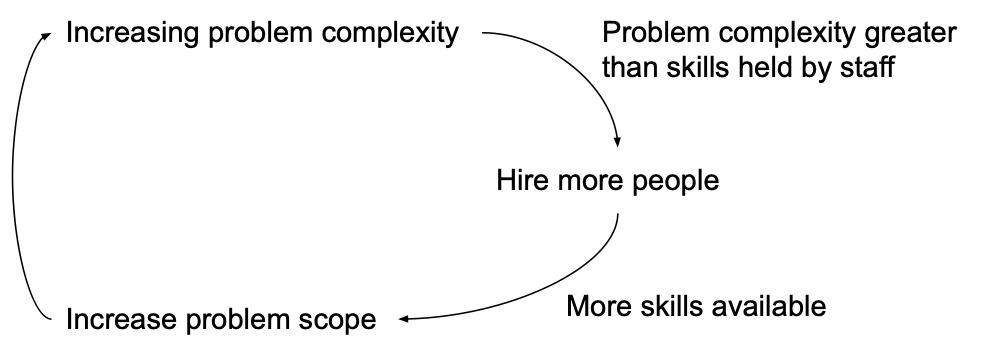
\includegraphics[width=0.8\textwidth]{images/feedback_loop_complexity_and_staffing}
    \caption{Increased complexity requires more staffing to enable specialization. More staff means more skills are available; under-utilized staff skills make room for more scope; more scope adds to complexity.}
    \label{fig:complexity_and_staff_growth}
\end{figure}
\end{center}


% claim: bureaucracy grow faster than the growth of human population?

Extrapolation of trends is easy: the more interconnected the society is, and with more people, and with more complicated products then more bureaucracy should be expected. If society reduces in size and reduces to tools we can make with only our hands then bureaucracy could decrease. 


\ \\

Since society might stay the same or get more interconnected for a while, learning about bureaucracy is a worthwhile investment. And if you want to reduce or eliminate bureaucracy, understanding what would be displaced is crucial. 
Happily, as described in the next chapter, you already have experience to build on. 